\documentclass[11pt]{article}
\usepackage[a4paper,margin=21mm]{geometry}
\usepackage[no-math]{fontspec}
\setmainfont{Latin Modern Roman}
\newfontfamily\CJKfont{Noto Serif CJK SC}
\XeTeXlinebreaklocale "zh"
\XeTeXlinebreakskip=0pt plus 1pt
\usepackage{amsmath,amssymb,amsthm,amscd,graphicx,color}
\usepackage{xurl}
\usepackage[unicode,hidelinks]{hyperref}
\allowdisplaybreaks
\setlength\emergencystretch{3em}
\numberwithin{equation}{section}
\usepackage{authblk,tikz,tkz-tab}


\numberwithin{equation}{section}

\newtheorem{Theorem}{Theorem}[section]
\newtheorem{Corollary}[Theorem]{Corollary}
\newtheorem{Lemma}[Theorem]{Lemma}
\newtheorem{Proposition}[Theorem]{Proposition}
 { \theoremstyle{definition}
\newtheorem{Definition}[Theorem]{Definition}
\newtheorem{Note}[Theorem]{Note}
\newtheorem{Example}[Theorem]{Example}
\newtheorem{Remark}[Theorem]{Remark}
\newtheorem{Notation}[Theorem]{Notation}}


\newcommand{\typ}[1]{\substack{\vspace{-2mm}\\ \begin{tikzpicture}[line cap=round,line join=round,>=triangle 45,x=0.7cm,y=0.7cm]
\clip(1.8,1.9) rectangle (2.2,2.7);
\draw [line width=.5pt,dash pattern=on #1pt off #1pt] (2.,2.5)-- (2.,2.);
\begin{scriptsize}
\end{scriptsize}
\end{tikzpicture}}}


\newcommand{\tun}{\begin{tikzpicture}[line cap=round,line join=round,>=triangle 45,x=0.5cm,y=0.5cm]
\clip(1.8,1.9) rectangle (2.2,2.2);
\begin{scriptsize}
\draw [fill=black] (2.,2.) circle (1pt);
\end{scriptsize}
\end{tikzpicture}}

\newcommand{\tdeux}[1]{\begin{tikzpicture}[line cap=round,line join=round,>=triangle 45,x=0.7cm,y=0.7cm]
\clip(1.8,1.9) rectangle (2.2,2.7);
\draw [line width=.5pt,dash pattern=on #1pt off #1pt] (2.,2.5)-- (2.,2.);
\begin{scriptsize}
\draw [fill=black] (2.,2.) circle (1pt);
\draw [fill=black] (2.,2.5) circle (1pt);
\end{scriptsize}
\end{tikzpicture}}

\newcommand{\ttroisun}[2]{\begin{tikzpicture}[line cap=round,line join=round,>=triangle 45,x=0.7cm,y=0.7cm]
\clip(1.5,1.9) rectangle (2.5,2.7);
\draw [line width=0.5pt,dash pattern=on #1pt off #1pt] (2.,2.)-- (1.7,2.5);
\draw [line width=0.5pt,dash pattern=on #2pt off #2pt] (2.,2.)-- (2.3,2.5);
\begin{scriptsize}
\draw [fill=black] (1.7,2.5) circle (1pt);
\draw [fill=black] (2.,2.) circle (1pt);
\draw [fill=black] (2.3,2.5) circle (1pt);
\end{scriptsize}
\end{tikzpicture}}
\newcommand{\ttroisdeux}{\begin{tikzpicture}[line cap=round,line join=round,>=triangle 45,x=0.7cm,y=0.7cm]
\clip(1.8,1.9) rectangle (2.2,3.2);
\draw [line width=0.5pt] (2.,2.5)-- (2.,2.);
\draw [line width=0.5pt] (2.,2.5)-- (2.,3.);
\begin{scriptsize}
\draw [fill=black] (2.,2.) circle (1pt);
\draw [fill=black] (2.,2.5) circle (1pt);
\draw [fill=black] (2.,3.) circle (1pt);
\end{scriptsize}
\end{tikzpicture}}

\newcommand{\tquatreun}{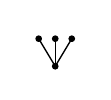
\begin{tikzpicture}[line cap=round,line join=round,>=triangle 45,x=0.7cm,y=0.7cm]
\clip(1.5,1.9) rectangle (2.5,2.7);
\draw [line width=0.5pt] (2.,2.)-- (1.7,2.5);
\draw [line width=0.5pt] (2.,2.)-- (2.3,2.5);
\draw [line width=0.5pt] (2.,2.)-- (2.,2.5);
\begin{scriptsize}
\draw [fill=black] (1.7,2.5) circle (1.0pt);
\draw [fill=black] (2.,2.) circle (1.0pt);
\draw [fill=black] (2.3,2.5) circle (1.0pt);
\draw [fill=black] (2.,2.5) circle (1.0pt);
\end{scriptsize}
\end{tikzpicture}}
\newcommand{\tquatredeux}{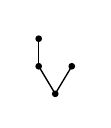
\begin{tikzpicture}[line cap=round,line join=round,>=triangle 45,x=0.7cm,y=0.7cm]
\clip(1.5,1.9) rectangle (2.5,3.2);
\draw [line width=0.5pt] (2.,2.)-- (1.7,2.5);
\draw [line width=0.5pt] (2.,2.)-- (2.3,2.5);
\draw [line width=0.5pt] (1.7,2.5)-- (1.7,3.);
\begin{scriptsize}
\draw [fill=black] (1.7,2.5) circle (1.0pt);
\draw [fill=black] (2.,2.) circle (1.0pt);
\draw [fill=black] (2.3,2.5) circle (1.0pt);
\draw [fill=black] (1.7,3.) circle (1.0pt);
\end{scriptsize}
\end{tikzpicture}}
\newcommand{\tquatretrois}{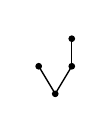
\begin{tikzpicture}[line cap=round,line join=round,>=triangle 45,x=0.7cm,y=0.7cm]
\clip(1.5,1.9) rectangle (2.5,3.2);
\draw [line width=0.5pt] (2.,2.)-- (1.7,2.5);
\draw [line width=0.5pt] (2.,2.)-- (2.3,2.5);
\draw [line width=0.5pt] (2.3,2.5)-- (2.3,3.);
\begin{scriptsize}
\draw [fill=black] (1.7,2.5) circle (1.0pt);
\draw [fill=black] (2.,2.) circle (1.0pt);
\draw [fill=black] (2.3,2.5) circle (1.0pt);
\draw [fill=black] (2.3,3.) circle (1.0pt);
\end{scriptsize}
\end{tikzpicture}}
\newcommand{\tquatrequatre}{\begin{tikzpicture}[line cap=round,line join=round,>=triangle 45,x=0.7cm,y=0.7cm]
\clip(1.5,1.9) rectangle (2.5,3.7);
\draw [line width=0.5pt] (2.,2.)-- (2.,2.5);
\draw [line width=0.5pt] (2.,2.5)-- (2.3,3.);
\draw [line width=0.5pt] (2.,2.5)-- (1.7,3.);
\begin{scriptsize}
\draw [fill=black] (2.,2.) circle (1.0pt);
\draw [fill=black] (2.,2.5) circle (1.0pt);
\draw [fill=black] (1.7,3.) circle (1.0pt);
\draw [fill=black] (2.3,3.) circle (1.0pt);
\end{scriptsize}
\end{tikzpicture}}
\newcommand{\tquatrecinq}{\begin{tikzpicture}[line cap=round,line join=round,>=triangle 45,x=0.7cm,y=0.7cm]
\clip(1.8,1.9) rectangle (2.5,3.7);
\draw [line width=0.5pt] (2.,2.)-- (2.,2.5);
\draw [line width=0.5pt] (2.,2.5)-- (2.,3.);
\draw [line width=0.5pt] (2.,3.)-- (2.,3.5);
\begin{scriptsize}
\draw [fill=black] (2.,2.) circle (1.0pt);
\draw [fill=black] (2.,2.5) circle (1.0pt);
\draw [fill=black] (2.,3.) circle (1.0pt);
\draw [fill=black] (2.,3.5) circle (1.0pt);
\end{scriptsize}
\end{tikzpicture}}

\newcommand{\tcinqun}{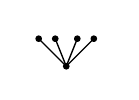
\begin{tikzpicture}[line cap=round,line join=round,>=triangle 45,x=0.7cm,y=0.7cm]
\clip(1.3,1.9) rectangle (2.8,2.7);
\draw [line width=0.5pt] (2.,2.)-- (1.5,2.5);
\draw [line width=0.5pt] (2.,2.)-- (1.8,2.5);
\draw [line width=0.5pt] (2.,2.)-- (2.2,2.5);
\draw [line width=0.5pt] (2.,2.)-- (2.5,2.5);
\begin{scriptsize}
\draw [fill=black] (1.5,2.5) circle (1.0pt);
\draw [fill=black] (1.8,2.5) circle (1.0pt);
\draw [fill=black] (2.2,2.5) circle (1.0pt);
\draw [fill=black] (2.5,2.5) circle (1.0pt);
\draw [fill=black] (2.,2.) circle (1.0pt);
\end{scriptsize}
\end{tikzpicture}}
\newcommand{\tcinqdeux}{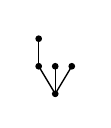
\begin{tikzpicture}[line cap=round,line join=round,>=triangle 45,x=0.7cm,y=0.7cm]
\clip(1.5,1.9) rectangle (2.5,3.2);
\draw [line width=0.5pt] (2.,2.)-- (1.7,2.5);
\draw [line width=0.5pt] (2.,2.)-- (2.3,2.5);
\draw [line width=0.5pt] (2.,2.)-- (2.,2.5);
\draw [line width=0.5pt] (1.7,2.5)-- (1.7,3.);
\begin{scriptsize}
\draw [fill=black] (1.7,2.5) circle (1.0pt);
\draw [fill=black] (2.,2.) circle (1.0pt);
\draw [fill=black] (2.,2.5) circle (1.0pt);
\draw [fill=black] (2.3,2.5) circle (1.0pt);
\draw [fill=black] (1.7,3.) circle (1.0pt);
\end{scriptsize}
\end{tikzpicture}}
\newcommand{\tcinqtrois}{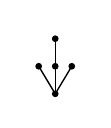
\begin{tikzpicture}[line cap=round,line join=round,>=triangle 45,x=0.7cm,y=0.7cm]
\clip(1.5,1.9) rectangle (2.5,3.2);
\draw [line width=0.5pt] (2.,2.)-- (1.7,2.5);
\draw [line width=0.5pt] (2.,2.)-- (2.3,2.5);
\draw [line width=0.5pt] (2.,2.)-- (2.,2.5);
\draw [line width=0.5pt] (2.,2.5)-- (2.,3.);
\begin{scriptsize}
\draw [fill=black] (1.7,2.5) circle (1.0pt);
\draw [fill=black] (2.,2.) circle (1.0pt);
\draw [fill=black] (2.,2.5) circle (1.0pt);
\draw [fill=black] (2.3,2.5) circle (1.0pt);
\draw [fill=black] (2.,3.) circle (1.0pt);
\end{scriptsize}
\end{tikzpicture}}
\newcommand{\tcinqquatre}{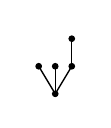
\begin{tikzpicture}[line cap=round,line join=round,>=triangle 45,x=0.7cm,y=0.7cm]
\clip(1.5,1.9) rectangle (2.5,3.2);
\draw [line width=0.5pt] (2.,2.)-- (1.7,2.5);
\draw [line width=0.5pt] (2.,2.)-- (2.3,2.5);
\draw [line width=0.5pt] (2.,2.)-- (2.,2.5);
\draw [line width=0.5pt] (2.3,2.5)-- (2.3,3.);
\begin{scriptsize}
\draw [fill=black] (1.7,2.5) circle (1.0pt);
\draw [fill=black] (2.,2.) circle (1.0pt);
\draw [fill=black] (2.,2.5) circle (1.0pt);
\draw [fill=black] (2.3,2.5) circle (1.0pt);
\draw [fill=black] (2.3,3.) circle (1.0pt);
\end{scriptsize}
\end{tikzpicture}}
\newcommand{\tcinqcinq}{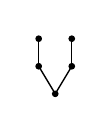
\begin{tikzpicture}[line cap=round,line join=round,>=triangle 45,x=0.7cm,y=0.7cm]
\clip(1.5,1.9) rectangle (2.5,3.2);
\draw [line width=0.5pt] (2.,2.)-- (1.7,2.5);
\draw [line width=0.5pt] (1.7,2.5)-- (1.7,3.);
\draw [line width=0.5pt] (2.,2.)-- (2.3,2.5);
\draw [line width=0.5pt] (2.3,2.5)-- (2.3,3.);
\begin{scriptsize}
\draw [fill=black] (1.7,2.5) circle (1.0pt);
\draw [fill=black] (2.,2.) circle (1.0pt);
\draw [fill=black] (1.7,3.) circle (1.0pt);
\draw [fill=black] (2.3,2.5) circle (1.0pt);
\draw [fill=black] (2.3,3.) circle (1.0pt);
\end{scriptsize}
\end{tikzpicture}}
\newcommand{\tcinqsix}{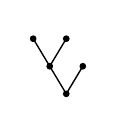
\begin{tikzpicture}[line cap=round,line join=round,>=triangle 45,x=0.7cm,y=0.7cm]
\clip(1.3,1.9) rectangle (2.5,3.2);
\draw [line width=0.5pt] (2.,2.)-- (1.7,2.5);
\draw [line width=0.5pt] (2.,2.)-- (2.3,2.5);
\draw [line width=0.5pt] (1.7,2.5)-- (1.4,3.);
\draw [line width=0.5pt] (1.7,2.5)-- (2,3.);
\begin{scriptsize}
\draw [fill=black] (1.7,2.5) circle (1.0pt);
\draw [fill=black] (2.,2.) circle (1.0pt);
\draw [fill=black] (2.3,2.5) circle (1.0pt);
\draw [fill=black] (1.4,3.) circle (1.0pt);
\draw [fill=black] (2.,3.) circle (1.0pt);
\end{scriptsize}
\end{tikzpicture}}
\newcommand{\tcinqsept}{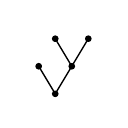
\begin{tikzpicture}[line cap=round,line join=round,>=triangle 45,x=0.7cm,y=0.7cm]
\clip(1.5,1.9) rectangle (2.8,3.2);
\draw [line width=0.5pt] (2.,2.)-- (1.7,2.5);
\draw [line width=0.5pt] (2.,2.)-- (2.3,2.5);
\draw [line width=0.5pt] (2.3,2.5)-- (2.6,3.);
\draw [line width=0.5pt] (2.3,2.5)-- (2,3.);
\begin{scriptsize}
\draw [fill=black] (1.7,2.5) circle (1.0pt);
\draw [fill=black] (2.,2.) circle (1.0pt);
\draw [fill=black] (2.3,2.5) circle (1.0pt);
\draw [fill=black] (2.6,3.) circle (1.0pt);
\draw [fill=black] (2.,3.) circle (1.0pt);
\end{scriptsize}
\end{tikzpicture}}
\newcommand{\tcinqhuit}{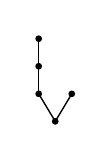
\begin{tikzpicture}[line cap=round,line join=round,>=triangle 45,x=0.7cm,y=0.7cm]
\clip(1.5,1.9) rectangle (2.5,3.7);
\draw [line width=0.5pt] (2.,2.)-- (1.7,2.5);
\draw [line width=0.5pt] (1.7,2.5)-- (1.7,3.);
\draw [line width=0.5pt] (2.,2.)-- (2.3,2.5);
\draw [line width=0.5pt] (1.7,3.)-- (1.7,3.5);
\begin{scriptsize}
\draw [fill=black] (1.7,2.5) circle (1.0pt);
\draw [fill=black] (2.,2.) circle (1.0pt);
\draw [fill=black] (1.7,3.) circle (1.0pt);
\draw [fill=black] (2.3,2.5) circle (1.0pt);
\draw [fill=black] (1.7,3.5) circle (1.0pt);
\end{scriptsize}
\end{tikzpicture}}
\newcommand{\tcinqneuf}{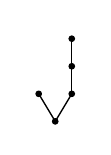
\begin{tikzpicture}[line cap=round,line join=round,>=triangle 45,x=0.7cm,y=0.7cm]
\clip(1.5,1.9) rectangle (2.5,3.7);
\draw [line width=0.5pt] (2.,2.)-- (1.7,2.5);
\draw [line width=0.5pt] (2.3,2.5)-- (2.3,3.);
\draw [line width=0.5pt] (2.,2.)-- (2.3,2.5);
\draw [line width=0.5pt] (2.3,3.)-- (2.3,3.5);
\begin{scriptsize}
\draw [fill=black] (1.7,2.5) circle (1.0pt);
\draw [fill=black] (2.,2.) circle (1.0pt);
\draw [fill=black] (2.3,3.) circle (1.0pt);
\draw [fill=black] (2.3,2.5) circle (1.0pt);
\draw [fill=black] (2.3,3.5) circle (1.0pt);
\end{scriptsize}
\end{tikzpicture}}
\newcommand{\tcinqdix}{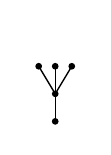
\begin{tikzpicture}[line cap=round,line join=round,>=triangle 45,x=0.7cm,y=0.7cm]
\clip(1.5,1.9) rectangle (2.5,3.7);
\draw [line width=0.5pt] (2.,2.)-- (2.,2.5);
\draw [line width=0.5pt] (2.,2.5)-- (2.3,3.);
\draw [line width=0.5pt] (2.,2.5)-- (1.7,3.);
\draw [line width=0.5pt] (2.,2.5)-- (2.,3.);
\begin{scriptsize}
\draw [fill=black] (2.,2.) circle (1.0pt);
\draw [fill=black] (2.,2.5) circle (1.0pt);
\draw [fill=black] (1.7,3.) circle (1.0pt);
\draw [fill=black] (2.3,3.) circle (1.0pt);
\draw [fill=black] (2.,3.) circle (1.0pt);
\end{scriptsize}
\end{tikzpicture}}
\newcommand{\tcinqonze}{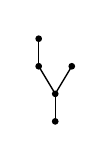
\begin{tikzpicture}[line cap=round,line join=round,>=triangle 45,x=0.7cm,y=0.7cm]
\clip(1.5,1.9) rectangle (2.5,3.7);
\draw [line width=0.5pt] (2.,2.)-- (2.,2.5);
\draw [line width=0.5pt] (2.,2.5)-- (2.3,3.);
\draw [line width=0.5pt] (2.,2.5)-- (1.7,3.);
\draw [line width=0.5pt] (1.7,3.)-- (1.7,3.5);
\begin{scriptsize}
\draw [fill=black] (2.,2.) circle (1.0pt);
\draw [fill=black] (2.,2.5) circle (1.0pt);
\draw [fill=black] (1.7,3.) circle (1.0pt);
\draw [fill=black] (2.3,3.) circle (1.0pt);
\draw [fill=black] (1.7,3.5) circle (1.0pt);
\end{scriptsize}
\end{tikzpicture}}
\newcommand{\tcinqdouze}{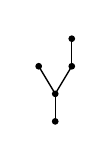
\begin{tikzpicture}[line cap=round,line join=round,>=triangle 45,x=0.7cm,y=0.7cm]
\clip(1.5,1.9) rectangle (2.5,3.7);
\draw [line width=0.5pt] (2.,2.)-- (2.,2.5);
\draw [line width=0.5pt] (2.,2.5)-- (2.3,3.);
\draw [line width=0.5pt] (2.,2.5)-- (1.7,3.);
\draw [line width=0.5pt] (2.3,3.)-- (2.3,3.5);
\begin{scriptsize}
\draw [fill=black] (2.,2.) circle (1.0pt);
\draw [fill=black] (2.,2.5) circle (1.0pt);
\draw [fill=black] (1.7,3.) circle (1.0pt);
\draw [fill=black] (2.3,3.) circle (1.0pt);
\draw [fill=black] (2.3,3.5) circle (1.0pt);
\end{scriptsize}
\end{tikzpicture}}
\newcommand{\tcinqtreize}{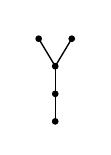
\begin{tikzpicture}[line cap=round,line join=round,>=triangle 45,x=0.7cm,y=0.7cm]
\clip(1.5,1.9) rectangle (2.5,3.7);
\draw [line width=0.5pt] (2.,2.)-- (2.,2.5);
\draw [line width=0.5pt] (2.,2.5)-- (2.,3.);
\draw [line width=0.5pt] (2.,3.)-- (1.7,3.5);
\draw [line width=0.5pt] (2.,3.)-- (2.3,3.5);
\begin{scriptsize}
\draw [fill=black] (2.,2.) circle (1.0pt);
\draw [fill=black] (2.,2.5) circle (1.0pt);
\draw [fill=black] (2.,3.) circle (1.0pt);
\draw [fill=black] (1.7,3.5) circle (1.0pt);
\draw [fill=black] (2.3,3.5) circle (1.0pt);
\end{scriptsize}
\end{tikzpicture}}
\newcommand{\tcinqquatorze}{\begin{tikzpicture}[line cap=round,line join=round,>=triangle 45,x=0.7cm,y=0.7cm]
\clip(1.8,1.9) rectangle (2.5,4.2);
\draw [line width=0.5pt] (2.,2.)-- (2.,2.5);
\draw [line width=0.5pt] (2.,2.5)-- (2.,3.);
\draw [line width=0.5pt] (2.,3.)-- (2.,3.5);
\draw [line width=0.5pt] (2.,3.5)-- (2.,4.);
\begin{scriptsize}
\draw [fill=black] (2.,2.) circle (1.0pt);
\draw [fill=black] (2.,2.5) circle (1.0pt);
\draw [fill=black] (2.,3.) circle (1.0pt);
\draw [fill=black] (2.,3.5) circle (1.0pt);
\draw [fill=black] (2.,4.) circle (1.0pt);
\end{scriptsize}
\end{tikzpicture}}

\newcommand{\tdun}[1]{\begin{tikzpicture}[line cap=round,line join=round,>=triangle 45,x=0.7cm,y=0.7cm]
\clip(1.8,1.9) rectangle (2.5,2.5);
\begin{scriptsize}
\draw [fill=black] (2.,2.) circle (1pt);
\end{scriptsize}
\draw(2.3,2.1) node {\tiny #1};
\end{tikzpicture}}

\newcommand{\tddeux}[3]{\begin{tikzpicture}[line cap=round,line join=round,>=triangle 45,x=0.7cm,y=0.7cm]
\clip(1.8,1.9) rectangle (2.5,3.);
\draw [line width=.5pt, dash pattern=on #3pt off #3pt] (2.,2.5)-- (2.,2.);
\begin{scriptsize}
\draw [fill=black] (2.,2.) circle (1pt);
\draw [fill=black] (2.,2.5) circle (1pt);
\end{scriptsize}
\draw(2.3,2.1) node {\tiny #1};
\draw(2.3,2.6) node {\tiny #2};
\end{tikzpicture}}

\newcommand{\tdtroisun}[5]{\begin{tikzpicture}[line cap=round,line join=round,>=triangle 45,x=0.7cm,y=0.7cm]
\clip(1.5,1.9) rectangle (2.5,3.2);
\draw [line width=0.5pt, dash pattern=on #4pt off #4pt] (2.,2.)-- (1.7,2.5);
\draw [line width=0.5pt, dash pattern=on #5pt off #5pt] (2.,2.)-- (2.3,2.5);
\begin{scriptsize}
\draw [fill=black] (1.7,2.5) circle (1pt);
\draw [fill=black] (2.,2.) circle (1pt);
\draw [fill=black] (2.3,2.5) circle (1pt);
\end{scriptsize}
\draw(2.4,2.1) node {\tiny #1};
\draw(2.3,2.8) node {\tiny #2};
\draw(1.7,2.8) node {\tiny #3};
\end{tikzpicture}}
\newcommand{\tdtroisdeux}[5]{\begin{tikzpicture}[line cap=round,line join=round,>=triangle 45,x=0.7cm,y=0.7cm]
\clip(1.8,1.9) rectangle (2.5,3.5);
\draw [line width=0.5pt, dash pattern=on #4pt off #4pt] (2.,2.5)-- (2.,2.);
\draw [line width=0.5pt, dash pattern=on #5pt off #5pt] (2.,2.5)-- (2.,3.);
\begin{scriptsize}
\draw [fill=black] (2.,2.) circle (1pt);
\draw [fill=black] (2.,2.5) circle (1pt);
\draw [fill=black] (2.,3.) circle (1pt);
\end{scriptsize}
\draw(2.3,2.1) node {\tiny #1};
\draw(2.3,2.6) node {\tiny #2};
\draw(2.3,3.1) node {\tiny #3};
\end{tikzpicture}}


\newcommand{\RF}{\mathcal{RF}}
\newcommand{\K}{\mathbb{K}}
\renewcommand{\L}{\mathcal{L}}
\newcommand{\A}{\K\langle\langle x_0,x_1\rangle\rangle}
\renewcommand{\AA}{\mathcal{A}}
\newcommand{\B}{\K\langle x_0,x_1\rangle}
\newcommand{\tcirc}{\tilde{\circ}}
\newcommand{\tdelta}{\tilde{\Delta}}
\newcommand{\T}{\mathcal{T}}
\newcommand{\F}{\mathcal{F}}
\newcommand{\C}{\mathcal{C}}
\newcommand{\D}{\mathcal{D}}
\newcommand{\PT}{\mathcal{PT}}
\newcommand{\UPT}{\mathcal{UPT}}
\newcommand{\g}{\mathfrak{g}}
\renewcommand{\S}{\mathfrak{S}}
\renewcommand{\PT}{\mathcal{PT}}
\newcommand{\N}{\mathbb{N}}
\newcommand{\adm}{\mathrm{Adm}}
\newcommand{\tdiam}{\tilde{\diamond}}
\newcommand{\tdiamd}{\tilde{\triangleleft}}
\newcommand{\U}{\mathcal{U}}
\newcommand{\h}{\mathcal{H}}
\newcommand{\bfDelta}{\mathbf{\Delta}}
\newcommand{\bftDelta}{\mathbf{\tdelta}}

\newcommand{\bfT}{\mathbb{T}}
\newcommand{\bfF}{\mathbb{F}}
\renewcommand{\P}{\mathcal{P}}
\newcommand{\M}{\mathcal{M}}
\newcommand{\NT}{N\mathbb{T}}
\newcommand{\NL}{N\mathbb{L}}

\newcommand{\dec}{\mathrm{dec}}
\newcommand{\id}{\mathrm{Id}}
\newcommand{\type}{\mathrm{type}}
\renewcommand{\ker}{\mathrm{Ker}}
\newcommand{\im}{\mathrm{Im}}

\newcommand{\rond}[1]{*++[o][F-]{#1}}
\usepackage[all]{xy}



\begin{document}
\begin{center}\Large The operad of multiple pre-Lie products indexed by a nonempty type set is the explicit rooted edge-typed tree operad\end{center}
\noindent\textbf{Stable ID:} 1432\quad\textbf{Author:} Loic Foissy\par
\noindent\textbf{Work:} Algebraic Structures on Typed Decorated Rooted Trees\par
\noindent\textbf{Source:} \url{https://sigma-journal.com/2021/086/}\par
\noindent\textbf{Version:} Official SIGMA 17 (2021) article 086, DOI 10.3842/SIGMA.2021.086; journal PDF and native TeX acquired 2026-09-30, exact bytes pinned by SHA256\par
\noindent\textbf{Rights:} CC BY 4.0. Authors retain copyright. \url{https://creativecommons.org/licenses/by/4.0/}. Reuse and typesetting adaptation; original language and mathematical content preserved.\par
\noindent\textbf{Difficulty (prior selection preserved):} {\CJKfont H2: The proof constructs the typed substitution operad and identifies its generators and cross-type pre-Lie relations. Surjectivity uses a double induction on vertex number and root fertility, while injectivity is obtained from an independently constructed free multiple pre-Lie algebra. The supporting construction descends a Guin-Oudom action through an explicitly controlled kernel and verifies the universal tree-grafting map.}\par
\medskip\noindent\textbf{Editorial boundary note (not author text):} Selected independent Theorem3.17 identifying the multiple pre-Lie operad with the explicit species operad of rooted edge-typed trees, over the stated characteristic-zero field and arbitrary nonempty type set. Full field/tree/forest/indexing conventions and complete typed grafting, formal-type pre-Lie extension, Guin-Oudom quotient-kernel descent, free universal tree algebra, two substitution associativity cases and both surjectivity/injectivity arguments are retained. Existing ordinary Guin-Oudom and standard species-operad definitions remain precise references; literal routine independence-of-scalar-map comment and source formula/index variants are preserved without an editor completion. Koszul-dual, enumeration, later freeness/Hopf/cointeraction outputs are unselected, with no supporting counts. All author tree drawings remain editable native TikZ. The original unused stmaryrd/mathabx/shuffle imports are omitted; retained body has no package-specific commands, and standard math notation is checked against the source PDF.\par
\medskip\hrule\medskip\noindent\textbf{Author text begins below.}\par
\setcounter{section}{1}
% Original source lines 469--495
We first define grafting products of trees, similar to the pre-Lie product of \cite{Chapoton}.
For any type $t$, we obtain a pre-Lie product $\bullet_t$ on the space $\g_{\D,\T}$ of $\T$-typed trees
whose vertices are decorated by elements of a set $\D$.
For example, if $\typ{10}$ and $\typ{2}$ are two types, if~$a, b,c\in \D$, then
\begin{gather*}
\tddeux{$a$}{$b$}{10}\bullet_{\typ{10}} \tdun{$c$}=
\tdtroisun{$a$}{$c$}{$b$}{10}{10}+\tdtroisdeux{$a$}{$b$}{$c$}{10}{10},\qquad\qquad
\tddeux{$a$}{$b$}{10}\bullet_{\typ{2}} \tdun{$c$}=
\tdtroisun{$a$}{$c$}{$b$}{10}{2}+\tdtroisdeux{$a$}{$b$}{$c$}{10}{2}.
\end{gather*}
Then $\g_{\D,\T}$, equipped with all these products, is a $\T$-multiple pre-Lie algebra
(Definition \ref{defi3}), also called matching pre-Lie algebras in \cite{GaoGuoZhang}:
for any types $t$ and $t'$, for any $x,y,z\in \g_{\D,\T}$,
\begin{gather*}
x\bullet_{t'}(y \bullet_t z)-(x\bullet_{t'} y)\bullet_t z=x\bullet_t(z \bullet_{t'} y)-(x\bullet_t z)\bullet_{t'} y.
\end{gather*}
This relation appears in \cite{BCCH}.
We prove in Corollary~\ref{cor9} that
it is the free $\T$-multiple pre-Lie algebra generated by $\D$, generalizing the result of~\cite{ChapotonLivernet},
first mentioned in \cite[Proposition~4.21]{BCCH}.
Consequently, we obtain a combinatorial description of the operad of $\T$-multiple pre-Lie algebras
in terms of $\T$-typed trees with indexed vertices (Theorem~\ref{theo11}): for example,
\begin{gather*}
\tddeux{$1$}{$2$}{10}\circ_1\tddeux{$1$}{$2$}{2}=\tdtroisun{$1$}{$3$}{$2$}{2}{10}
+\tdtroisdeux{$1$}{$2$}{$3$}{2}{10},\qquad\qquad
\tddeux{$1$}{$2$}{2}\circ_2\tddeux{$1$}{$2$}{10}=\tdtroisdeux{$1$}{$2$}{$3$}{2}{10}.
\end{gather*}

\setcounter{Theorem}{0}
% Original source lines 579--686
\begin{Notation}\qquad
\begin{itemize}\itemsep=0pt
\item We denote by $\K$ a commutative field of characteristic zero. All the objects (vector spaces, algebras,
 coalgebras, pre-Lie algebras, $\dots$)
in this text will be taken over $\K$.
\item For any $n\in \mathbb{N}$, we denote by $[n]$ the set $\{1,\dots,n\}$.
\item For any set $\T$, we denote by $\K^\T$ the set of family $\lambda=(\lambda_t)_{t\in \T}$ of elements of $\K$
indexed by~$\T$, and we denote by $\K^{(\T)}$ the set of elements $\lambda\in \K^\T$ with a finite support.
Note that if~$\T$ is finite, then $\K^\T=\K^{(\T)}$.
\end{itemize}
\end{Notation}

\section{Typed decorated trees}

\subsection{Definition}

\begin{Definition}
Let $\D$ and $\T$ be two nonempty sets.
\begin{enumerate}\itemsep=0pt
\item A $\D$-decorated $\T$-typed forest is a triple $(F,\dec,\type)$, where
\begin{itemize}\itemsep=0pt
\item $F$ is a rooted forest. The set of its vertices is denoted by $V(F)$ and the set of its edges by $E(F)$.
\item $\dec\colon V(F)\longrightarrow \D$ is a map.
\item $\type\colon E(F)\longrightarrow \T$ is a map.
\end{itemize}
If the underlying rooted forest of $F$ is connected, we shall say that $F$ is a $\D$-decorated $\T$-typed tree.
\item If $(F,\dec_F,\type_F)$ and $(G,\dec_G,\type_G)$ are two $\D$-decorated $\T$-typed forests,
they are isomorphic if there exists a rooted forest isomorphism $f$ from $F$ to $G$ such that for any vertex $v$ of $F$,
$\dec_G(f(v))=\dec_F(v)$ and for any edge $e$ of $F$, $\type_G(f(e))=\type_F(e)$
\item For any finite set $A$, we denote by $\bfT_\T(A)$ the set of $A$-decorated
$\T$-typed trees $T$ such that $V(T)=A$
and $\dec=\id_A$, and by $\bfF_\T(A)$ the set of $A$-decorated $\T$-typed forests $F$ such that $V(F)=A$ and $\dec=\id_A$.
\item For any $n\geq 0$, we denote by $\bfT_{\D,\T}(n)$ the set of isomorphism classes of $\D$-decorated $\T$-typed trees $T$
such that $|V(T)|=n$ and by $\bfF_{\D,\T}(n)$ the set of isomorphism classes of $\D$-decorated $\T$-typed forests $F$
such that $|V(F)|=n$.
We also put
\begin{gather*}
\bfT_{\D,\T}=\bigsqcup_{n\geq 0} \bfT_{\D,\T}(n),\qquad
\bfF_{\D,\T}=\bigsqcup_{n\geq 0} \bfF_{\D,\T}(n).
\end{gather*}
\end{enumerate}
\end{Definition}

\begin{Example}
We shall represent the decorations of the vertices by letters alongside them.
If~$\T$ contains two elements, represented by $\typ{10}$ and $\typ{2}$\!, then
\begin{gather*}
\bfF_{\D,\T}(1)=\{\tdun{$d$},d\in \D\},
\\
\bfF_{\D,\T}(2)=\begin{Bmatrix}
\tdun{$a$}\tdun{$b$},\tddeux{$a$}{$b$}{10},\tddeux{$a$}{$b$}{2}, a,b\in \D
\end{Bmatrix}\!,
\\
\bfF_{\D,\T}(3)=\begin{Bmatrix}
\tdun{$a$}\tdun{$b$}\tdun{$c$},\tddeux{$a$}{$b$}{10}\tdun{$c$},\tddeux{$a$}{$b$}{2}\tdun{$c$},
\tdtroisun{$a$}{$c$}{$b$}{10}{10},\tdtroisun{$a$}{$c$}{$b$}{2}{10},\tdtroisun{$a$}{$c$}{$b$}{2}{2},
\tdtroisdeux{$a$}{$b$}{$c$}{10}{10},\tdtroisdeux{$a$}{$b$}{$c$}{2}{10},
\tdtroisdeux{$a$}{$b$}{$c$}{10}{2},\tdtroisdeux{$a$}{$b$}{$c$}{2}{2}, a,b,c\in \D\end{Bmatrix}\!.
\end{gather*}
Note that for any $a$, $b$, $c\in \D$,
\begin{gather*}
\tdun{$a$}\tdun{$b$}=\tdun{$b$}\tdun{$a$},\qquad\qquad
\tdtroisun{$a$}{$c$}{$b$}{10}{10}=\tdtroisun{$a$}{$b$}{$c$}{10}{10},\qquad\qquad
\tdtroisun{$a$}{$c$}{$b$}{10}{2}=\tdtroisun{$a$}{$b$}{$c$}{2}{10},\qquad\qquad
\tdtroisun{$a$}{$c$}{$b$}{2}{2}=\tdtroisun{$a$}{$b$}{$c$}{2}{2}.
\end{gather*}
Moreover,
\begin{gather*}
\bfF_{\D,\T}([1])=\{\tdun{$1$}\},
\\
\bfF_{\D,\T}([2])=\begin{Bmatrix}\tdun{$1$}\tdun{$2$},
\tddeux{$1$}{$2$}{10},\tddeux{$2$}{$1$}{10},\tddeux{$1$}{$2$}{2},\tddeux{$2$}{$1$}{2}\end{Bmatrix}\!,
\\
\bfF_{\D,\T}([3])=\left\{\!\!\begin{array}{l}
\tdun{$1$}\tdun{$2$}\tdun{$3$},
\tddeux{$1$}{$2$}{10}\tdun{$3$},\tddeux{$1$}{$3$}{10}\tdun{$2$},\tddeux{$2$}{$1$}{10}\tdun{$3$},
\tddeux{$2$}{$3$}{10}\tdun{$1$},\tddeux{$3$}{$1$}{10}\tdun{$2$},\tddeux{$3$}{$2$}{10}\tdun{$1$},
\\
\tddeux{$1$}{$2$}{2}\tdun{$3$},\tddeux{$1$}{$3$}{2}\tdun{$2$},\tddeux{$2$}{$1$}{2}\tdun{$3$},
\tddeux{$2$}{$3$}{2}\tdun{$1$},\tddeux{$3$}{$1$}{2}\tdun{$2$},\tddeux{$3$}{$2$}{2}\tdun{$1$},
\\
\tdtroisun{$1$}{$3$}{$2$}{10}{10},\tdtroisun{$2$}{$3$}{$1$}{10}{10},\tdtroisun{$3$}{$2$}{$1$}{10}{10},
\tdtroisun{$1$}{$3$}{$2$}{2}{10},\tdtroisun{$1$}{$2$}{$3$}{2}{10},\tdtroisun{$2$}{$3$}{$1$}{2}{10},
\tdtroisun{$2$}{$1$}{$3$}{2}{10},\tdtroisun{$3$}{$2$}{$1$}{2}{10},\tdtroisun{$3$}{$1$}{$2$}{2}{10},
\tdtroisun{$1$}{$3$}{$2$}{2}{2},\tdtroisun{$2$}{$3$}{$1$}{2}{2},
\tdtroisun{$3$}{$2$}{$1$}{2}{2},\\
\tdtroisdeux{$1$}{$2$}{$3$}{10}{10},\tdtroisdeux{$1$}{$3$}{$2$}{10}{10},\tdtroisdeux{$2$}{$1$}{$3$}{10}{10},
\tdtroisdeux{$2$}{$3$}{$1$}{10}{10},\tdtroisdeux{$3$}{$1$}{$2$}{10}{10},\tdtroisdeux{$3$}{$2$}{$1$}{10}{10},
\tdtroisdeux{$1$}{$2$}{$3$}{2}{10},\tdtroisdeux{$1$}{$3$}{$2$}{2}{10},
\tdtroisdeux{$2$}{$1$}{$3$}{2}{10},\tdtroisdeux{$2$}{$3$}{$1$}{2}{10},
\tdtroisdeux{$3$}{$1$}{$2$}{2}{10},\tdtroisdeux{$3$}{$2$}{$1$}{2}{10},
\\
\tdtroisdeux{$1$}{$2$}{$3$}{10}{2},\tdtroisdeux{$1$}{$3$}{$2$}{10}{2},
\tdtroisdeux{$2$}{$1$}{$3$}{10}{2},\tdtroisdeux{$2$}{$3$}{$1$}{10}{2},
\tdtroisdeux{$3$}{$1$}{$2$}{10}{2},\tdtroisdeux{$3$}{$2$}{$1$}{10}{2},
\tdtroisdeux{$1$}{$2$}{$3$}{2}{2},\tdtroisdeux{$1$}{$3$}{$2$}{2}{2},
\tdtroisdeux{$2$}{$1$}{$3$}{2}{2},\tdtroisdeux{$2$}{$3$}{$1$}{2}{2},
\tdtroisdeux{$3$}{$1$}{$2$}{2}{2},\tdtroisdeux{$3$}{$2$}{$1$}{2}{2}
\end{array}\!\!\right\}\!.
\end{gather*}
\end{Example}

\begin{Remark}
If $|\T|=1$, all the edges of elements of $\bfF_{\D,\T}$ have the same type:
we work with $\D$-decorated rooted forests.
In this case, we shall omit $\T$ in the indices describing the forests, trees, spaces we are considering.
\end{Remark}



% Original source lines 752--1202
\section{Multiple pre-Lie algebras}

We here fix a nonempty set $\T$ of edges types.

\subsection{Definition}

\begin{Definition} \label{defi3}
A $\T$-multiple pre-Lie algebra is a family $(V,(\bullet_t)_{t\in \T})$,
where $V$ is a vector space and for all $t\in \T$,
$\bullet_t$ is a bilinear product on $V$ such that
\begin{gather*}
\forall t,t'\in \T,\quad\forall x,y,z\in V,\qquad
x\bullet_{t'}(y \bullet_t z)-(x\bullet_{t'} y)\bullet_t z=x\bullet_t(z \bullet_{t'} y)-(x\bullet_t z)\bullet_{t'} y.
\end{gather*}
\end{Definition}

\begin{Remark}
For any $t\in \T$, $(V,\bullet_t)$ is a pre-Lie algebra.
More generally, for any family $\lambda=(\lambda_t)_{t\in \T}\in \K^{(\T)}$,
putting $\bullet_\lambda=\sum \lambda_t \bullet_t$, $(V,\bullet_\lambda)$ is a pre-Lie algebra.
\end{Remark}

\begin{Proposition}
Let $\D$ be any set; we denote by $\g_{\D,\T}$ the vector space generated by $\bfT_{\D,\T}$.
For any $T,T'\in \bfT_{\D,\T}$,
$v\in V(T)$ and $t\in \T$, we denote by $T\bullet_t^{(v)} T'$ the $\D$-decorated $\T$-typed tree
obtained by grafting $T'$ on $v$ $($that is to say adding an edge between $v$ and the root of $T')$, the created edge being of type $t$.
We then define a product $\bullet_t$ on $\g_{\D,\T}$ by
\begin{gather*}
\forall T,T'\in \bfT_{\D,\T},\qquad
T\bullet_t T'=\sum_{v\in V(T)} T\bullet_t^{(v)} T'.
\end{gather*}
Then $(\g_{\D,\T},(\bullet_t)_{t\in \T})$ is a $\T$-multiple pre-Lie algebra.
\end{Proposition}

\begin{proof} Let $T$, $T'$, $T''$ be elements of $\bfT_{\D,\T}$ and $t',t''\in \T$.
\begin{gather*}
(T\bullet_{t'} T')\bullet_{t''} T''-T\bullet_{t'}(T'\bullet_{t''}T'')
\\ \qquad
{}=\sum_{v\in V(T), v'\in V(T)\sqcup V(T')} \big(T\bullet_{t'}^{(v)} T'\big)\bullet_{t''}^{(v')} T''
-\sum_{v\in V(T),v'\in V(T')}T\bullet_{t'}^{(v)}\big(T'\bullet_{t''}^{(v')} T''\big)
\\ \qquad
{}=\sum_{v\in V(T), v'\in V(T)}\!\!\!\!\!\! \big(T\bullet_{t'}^{(v)} T'\big)\bullet_{t''}^{(v')} T''
\!+\!\!\!\sum_{v\in V(T),v'\in V(T')}\!\!\!\!\!\!\big(T\bullet_{t'}^{(v)} T'\big)\bullet_{t''}^{(v')} T''
\!-T\bullet_{t'}^{(v)}\!\big(T'\bullet_{t''}^{(v')} T''\big)
\\ \qquad
{}=\sum_{v\in V(T), v'\in V(T)} \big(T\bullet_{t'}^{(v)} T'\big)\bullet_{t''}^{(v')} T''
\\ \qquad
{}=\sum_{v\in V(T), v'\in V(T)} \big(T\bullet_{t''}^{(v')} T''\big)\bullet_{t'}^{(v)} T'
\\ \qquad
{}=(T\bullet_{t''} T'')\bullet_{t'} T'-T\bullet_{t''}(T''\bullet_{t'}T').
\end{gather*}
So $\g_{\D,\T}$ is indeed a $\T$-multiple pre-Lie algebra.
\end{proof}

\begin{Example} If $a,b,c\in \D$ and $\typ{10}$\!, $\typ{2} \in \T$,\vspace{-1ex}
\begin{gather*}
\tddeux{$a$}{$b$}{10}\bullet_{\typ{10}} \tdun{$c$}=
\tdtroisun{$a$}{$c$}{$b$}{10}{10}+\tdtroisdeux{$a$}{$b$}{$c$}{10}{10},\qquad\qquad
\tddeux{$a$}{$b$}{10}\bullet_{\typ{2}} \tdun{$c$}=
\tdtroisun{$a$}{$c$}{$b$}{10}{2}+\tdtroisdeux{$a$}{$b$}{$c$}{10}{2}.
\end{gather*}\end{Example}


\subsection{Guin--Oudom extension of the pre-Lie products}

{\samepage\begin{Notation}
Let $(\partial_t)_{t\in \T}$ be a family of formal symbols indexed by $\T$. For any vector space~$V$, we denote
\begin{gather*}
V^{\oplus \T}=V\otimes \mathrm{Vect}(\partial_t,\:t\in \T).
\end{gather*}
Then
\begin{gather*}
V^{\oplus \T}=\bigoplus_{t\in \T} V\otimes \partial_t.
\end{gather*}
\end{Notation}
In order to enlighten the notations, we write $v\partial_t$ instead of $v\otimes \partial_t$
for any $v\in V$ and for any $t\in \T$.

}

\begin{Lemma}
If for any $t\in \T$, $\bullet_t$ is a bilinear product on a vector space $V$,
we define $\bullet\,{:}$ $\big(V^{\oplus \T}\big)^{\otimes 2}\longrightarrow V^{\oplus \T}$ by
\begin{gather*}
x\partial_t \bullet x'\partial_{t'}=(x\bullet_{t'} y)\partial_t.
\end{gather*}
Then $(V,(\bullet_t)_{t\in \T})$ is a $\T$-multiple pre-Lie algebra if,
and only if, $\big(V^{\oplus \T},\bullet\big)$ is a pre-Lie algebra.
\end{Lemma}

\begin{proof}
Let $x,x',x''\in V$, $t,t',t''\in \T$. Then
\begin{gather*}
x\partial_t\bullet (x'\partial_{t'}\bullet x''\partial_{t''})-(x\partial_t\bullet x'\partial_{t'})\bullet x''\partial_{t''}
=\left((x\bullet_{t'} x')\bullet_{t''} x''-x\bullet_{t'}(x'\bullet_{t''}x'')\right)\partial_t,
\end{gather*}
which implies the result.
\end{proof}

\begin{Notation}
The symmetric algebra $S(V)$ is given with its usual coproduct $\Delta$, making it a~bialgebra:
\begin{gather*}
\forall x\in V,\qquad \Delta(x)=x\otimes 1+1\otimes x.
\end{gather*}
We shall use Sweedler's notation: for any $w\in S(V)$, $\Delta(w)=\sum w^{(1)}\otimes w^{(2)}$.
The counit of this coproduct is denoted by $\varepsilon$: this is the unique algebra morphism from $S(V)$ to $\K$ sending any $v\in V$ to $0$.
\end{Notation}

\begin{Theorem}
Let $V$ be a $\T$-multiple pre-Lie algebra. One can define a product
\begin{gather*}
\bullet\colon\ S(V)\otimes S\big(V^{\oplus\T}\big)\longrightarrow S(V)
\end{gather*}
in the following way: for any $u,v \in S(V)$, $w\in S\big(V^{\oplus\T}\big)$, $x\in V$, $t\in \T$,
\begin{gather*}
1\bullet w=\varepsilon(w),
\\
u\bullet 1=u,
\\
uv\bullet w=\sum\big(u\bullet w^{(1)}\big)\big(v\bullet w^{(2)}\big),
\\
u\bullet w (x\partial_t)=(u\bullet w)\bullet_t x-x\bullet (w\bullet_t x),
\end{gather*}
where $\bullet_t$ is extended to $S(V)\otimes V$ and $S\big(V^{\oplus\T}\big)\otimes V$
by the following: for any $x_1,\dots,x_k,x\in V$, for any $t_1,\dots,t_k \in \T$,
\begin{gather*}
x_1\cdots x_k \bullet_t x=\sum_{i=1}^k x_1\cdots (x_i\bullet_t x)\cdots x_k,
\\
(x_1\partial_{t_1})\cdots (x_k\partial_{t_k}) \bullet_t x
=\sum_{i=1}^k (x_1\partial_{t_1})\cdots ((x_i\bullet_t x)\partial_{t_i})\cdots (x_k\partial_{t_k}).
\end{gather*}
\end{Theorem}

\begin{proof} \textit{Uniqueness}. The last formula allows to compute $x\bullet w$ for any $x\in V$
and $w\in S\big(V^{\oplus\T}\big)$ by induction on the length of $w$;
the other ones allow to compute $u\bullet w$ for any $u\in S(V)$ by induction on the length on $u$.
So this product $\bullet$ is unique.

\textit{Existence}. Let us use the Guin--Oudom construction \cite{Guin1,Guin2} on the pre-Lie algebra $V^{\otimes \T}$.
We obtain a product $\bullet$
defined on $S\big(V^{\oplus\T}\big)$ such that for any $u,v,w\in S\big(V^{\oplus\T}\big)$, $x\in V^{\oplus \T}$:
\begin{gather*}
1\bullet w=\varepsilon(w),
\\
u\bullet 1=u,
\\
uv\bullet w=\sum \big(u\bullet w^{(1)}\big)\big(v\bullet w^{(2)}\big),
\\
u\bullet w x=(u\bullet w)\bullet x-x\bullet (w\bullet x).
\end{gather*}
Let $f\colon \T\longrightarrow \K$ be any nonzero map. We consider the surjective algebra morphism
$F\colon S\big(V^{\oplus\T}\big)\allowbreak\longrightarrow S(V)$,
sending $x\partial_t$ to $f(t)x$ for any $x\in V$, $t\in \T$. Its kernel is generated by the elements
$X_{t,t'}x=(f(t')\partial_t-f(t)\partial_{t'})x$,
where $x\in V$ and $t,t'\in \T$. We denote by $J$ the vector space generated by the elements $X_{t,t'}x$.
Let us prove that for any $w\in S\big(V^{\oplus\T}\big)$, $J\bullet w\subseteq J$ by induction on the length $n$ of $w$.
If $n=0$, we can assume that $w=1$ and this is obvious. If $n=1$, we can assume that $w=x'\partial_{t''}$. Then
\begin{gather*}
X_{t,t'}x\bullet w=(f(t')\partial_t-f(t)\partial_{t'}) x\bullet_{t''} x'
=X_{t,'t'}x\bullet_{t''} x' \in J.'
\end{gather*}
Let us assume the result at rank $n-1$. We can assume that $w=w' x'\partial_t$, the length of $w'$ being $n-1$.
For any $x\in J$,
\begin{gather*}
x\bullet w=(x\bullet w')\bullet x'-x\bullet(w'\bullet x').
\end{gather*}
The length of $w'$ and $w'\bullet x'$ is $n-1$, so $x\bullet w'$ and $x\bullet (w'\bullet x')$ belong to $J$.
From the case $n=1$,
$(x\bullet w')\bullet x'\in J$, so $x\bullet w\in J$.

For any $x\in J$, $u,v\in S\big(V^{\oplus\T}\big)$,
\begin{gather*}
xu\bullet v=\underbrace{\big(x\bullet v^{(1)}\big)}_{\in J} \big(u\bullet v^{(2)}\big) \in \ker(F).
\end{gather*}
This proves that $\ker(F)\bullet S\big(V^{\oplus\T}\big)\subseteq \ker(F)$. Hence, $\bullet$ induces a product also denoted by $\bullet$,
defined from $S(V)\otimes S\big(V^{\otimes \T}\big)$ to $S(V)$. It is not difficult to show that it does not depend on the choice of $f$
and satisfies the required properties.
\end{proof}

\begin{Definition}
Let $d\in \D$, $T_1,\dots,T_k\in \bfT_{\D,\T}$, $t_1,\dots,t_k\in \T$. We denote by
\begin{gather*}
B_d\bigg(\prod_{i\in [k]} T_i\partial_{t_i}\bigg)
\end{gather*}
the $\T$-typed $\D$-decorated tree obtained by grafting $T_1,\dots,T_k$ on a common root decorated by~$d$,
the edge between this root and the root of $T_i$ being of type $t_i$ for any~$i$.
This defines a map $B_d\colon S\left(\mathrm{Vect}(\bfT_{\D,\T})^{\oplus \T}\right)\longrightarrow S(\mathrm{Vect}(\bfT_{\D,\T}))$.
\end{Definition}

\begin{Lemma} \label{lemma8}
For any $d\in \D$, $T_1,\dots,T_k\in \bfT_{\D,\T}$, $t_1,\dots,t_k\in \T$,
\begin{gather*}
B_d\bigg(\prod_{i\in [k]} T_i\partial_{t_i}\bigg)=\tdun{$d$}\bullet\prod_{i\in [k]} T_i\partial_{t_i}.
\end{gather*}
\end{Lemma}

\begin{proof} We write $F=\prod_{i\in [k]} T_i\partial_{t_i}$: the integer $k$ is unique
and denoted by $\ell(F)$. We proceed by induction on $\ell(F)$.
If $\ell(F)=0$, then $F=1$ and $\tdun{$d$}\bullet 1=\tdun{$d$}=B_d(1)$.
let us assume the result for any forest $F'$ with $\ell(F')=\ell(F)-1$. Putting $k=\ell(F)$,
we can write $F=F'T\partial_t$, with $\ell(F')=\ell(F)-1$, $T=T_k$ and $t=t_k$. Then
\begin{align*}
\tdun{$d$}\bullet F&=(\tdun{$d$}\bullet F')\bullet T\partial_t-\tdun{$d$}\bullet (F'\bullet T\partial_t)\\
&=B_d(F')\bullet_t T-B_d(F'\bullet_t T)\\
&=B_d(F'T\partial_t)+B_d(F'\bullet_t T)-B_d(F'\bullet_t T)\\
&=B_d(F).
\end{align*}
So the result holds for all forests. \end{proof}

\begin{Corollary} \label{cor9}
Let $A$ be a $\T$-multiple pre-Lie algebra and, for any $d\in \D$, $a_d \in A$.
There exists a unique $\T$-multiple algebra morphism
$\phi\colon \g_{\D,\T}\longrightarrow A$, such that for any $d\in \D$, $\phi(\tdun{$d$})=a_d$.
In~other words, $\g_{\T,\D}$ is the free $\T$-multiple pre-Lie algebra generated by $\D$.
\end{Corollary}

\begin{proof} \textit{Uniqueness}. Using the Guin--Oudom product and lemma \ref{lemma8},
$\phi$ is the unique linear map inductively defined by
\begin{gather*}
\phi\bigg(B_d\bigg(\prod_{i\in[k]}T_i \partial_{t_i}\bigg)\bigg)
=a_d \bullet \prod_{i\in [k]} \phi(T_i) \partial_{t_i}.
\end{gather*}

\textit{Existence}. Let $T,T'\in \bfT_{\D,\T}$ and $t\in \T$. Let us prove that $\phi(T\bullet_t T')=\phi(T)\bullet_t \phi(T')$
by induction on $n=|T|$. If $n=1$, we assume that $T=\tdun{$d$}$. Then $T\bullet_t T'=B_d(T'\partial_t)$, so
\begin{gather*}
\phi(T\bullet_t T')=a_d\bullet (\phi(T')\partial_t=a_d \bullet_t \phi(T')=\phi(T)\bullet_t \phi(T').
\end{gather*}
Let us assume the result at all ranks $<|T|$. We put
\begin{gather*}
T=B_d\bigg(\prod_{i=1}^k T_i\partial_{t_i}\bigg).
\end{gather*}
By definition of the pre-Lie product of $\g_{\D,\T}$ in terms of grafting,
\begin{gather*}
T\bullet T'=B_d\bigg(\prod_{i=1}^k T_i \partial_{t_i} T'\partial_t\bigg)+\sum_{j=1}^k B_d\bigg(\prod_{i\neq j} T_i\partial_{t_i} (T_j\bullet_t T')\partial_{t_j}\bigg),
\\
\phi(T\bullet T')=a_d\bullet \prod_{i=1}^k \phi(T_i)\partial_{t_i}\phi(T')\partial_t
+\sum_{j=1}^k a_d\bullet \prod_{i\neq j} \phi(T_i)\partial_{t_i} (\phi(T_j\bullet_t T'))\partial_{t_j}
\\ \hphantom{\phi(T\bullet T')}
{}=a_d\bullet \prod_{i=1}^k \phi(T_i)\partial_{t_i}\phi(T')\partial_t
+\sum_{j=1}^k a_d\bullet \prod_{i\neq j} \phi(T_i)\partial_{t_i} (\phi(T_j)\bullet_t \phi(T'))\partial_{t_j}
\\ \hphantom{\phi(T\bullet T')}
{}=a_d\bullet \prod_{i=1}^k \phi(T_i)\partial_{t_i}\phi(T')\partial_t+a_d\bullet\bigg(\bigg(\prod_{i=1}^k
\phi(T_i)\partial_{t_i}\bigg)\bullet \phi(T')\partial_t\bigg)
\\ \hphantom{\phi(T\bullet T')}
{}=\bigg(a_d\bullet\prod_{i=1}^k \phi(T_i)\partial_{t_i} \bigg)\bullet \phi(T')\partial_t
\\ \hphantom{\phi(T\bullet T')}
{}=\phi(T)\bullet_t \phi(T').
\end{gather*}
So $\phi$ is a $\T$-multiple pre-Lie algebra morphism. \end{proof}

\subsection{Operad of typed trees}

We now describe an operad of typed trees, in the category of species.
We refer to \cite{Dotsenko,Vallette,Markl} for notations and definitions on operads.

\begin{Notation} Let $A$ be a finite set. If $T\in \bfT_\T(A)$ and $a\in T$:
\begin{enumerate}\itemsep=0pt
\item The subtrees formed by the connected components of the set of vertices, descendants of~$a$ ($a$ excluded)
are denoted by $T_1^{(a)},\dots,T_{n_a}^{(a)}$.
The type of the edge from $a$ to the root of~$T_i^{(a)}$ is denoted by $t_i$.
\item The tree formed by the vertices of $T$ which are not in $T_1^{(a)},\dots,T_{n_a}^{(a)}$,
at the exception of~$a$, is denoted by $T_0^{(a)}$.
\end{enumerate}
\end{Notation}

\begin{Example}
Let us consider the following tree:\vspace{-1ex}
\begin{gather*}T
=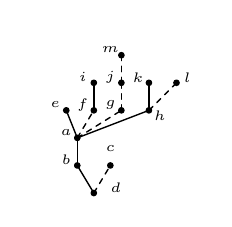
\begin{tikzpicture}[line cap=round,line join=round,>=triangle 45,x=0.7cm,y=0.7cm]
\clip(0.8,1.9) rectangle (4.,5.);
\draw [line width=0.5pt] (2.,2.)-- (1.7,2.5);
\draw [line width=0.5pt, dash pattern=on 2pt off 2pt] (2.,2.)-- (2.3,2.5);
\draw [line width=0.5pt] (1.7,2.5)-- (1.7,3.);
\draw [line width=0.5pt] (1.7,3.)-- (1.5,3.5);
\draw [line width=0.5pt, dash pattern=on 2pt off 2pt] (1.7,3.)-- (2.,3.5);
\draw [line width=0.5pt, dash pattern=on 2pt off 2pt] (1.7,3.)-- (2.5,3.5);
\draw [line width=0.5pt] (1.7,3.)-- (3.,3.5);
\draw [line width=0.5pt] (2.,3.5)-- (2.,4.);
\draw [line width=0.5pt, dash pattern=on 2pt off 2pt] (2.5,3.5)-- (2.5,4.);
\draw [line width=0.5pt] (3.,3.5)-- (3.,4.);
\draw [line width=0.5pt, dash pattern=on 2pt off 2pt] (3.,3.5)-- (3.5,4.);
\draw [line width=0.5pt, dash pattern=on 2pt off 2pt] (2.5,4.)-- (2.5,4.5);
\begin{scriptsize}
\draw [fill=black] (1.7,2.5) circle (1pt);
\draw [fill=black] (2.,2.) circle (1pt);
\draw [fill=black] (2.3,2.5) circle (1pt);
\draw [fill=black] (1.7,3.) circle (1pt);
\draw [fill=black] (1.5,3.5) circle (1pt);
\draw [fill=black] (2.,3.5) circle (1pt);
\draw [fill=black] (2.5,3.5) circle (1pt);
\draw [fill=black] (3.,3.5) circle (1pt);
\draw [fill=black] (2.,4.) circle (1pt);
\draw [fill=black] (2.5,4.) circle (1pt);
\draw [fill=black] (3.,4.) circle (1pt);
\draw [fill=black] (3.5,4.) circle (1pt);
\draw [fill=black] (2.5,4.5) circle (1pt);
\end{scriptsize}
\draw(2.4,2.1) node {\tiny $d$};
\draw(2.3,2.8) node {\tiny $c$};
\draw(1.5,2.6) node {\tiny $b$};
\draw(1.5,3.1) node {\tiny $a$};
\draw(1.3,3.6) node {\tiny $e$};
\draw(1.8,3.6) node {\tiny $f$};
\draw(2.3,3.6) node {\tiny $g$};
\draw(3.2,3.4) node {\tiny $h$};
\draw(1.8,4.1) node {\tiny $i$};
\draw(2.3,4.1) node {\tiny $j$};
\draw(2.8,4.1) node {\tiny $k$};
\draw(3.7,4.1) node {\tiny $l$};
\draw(2.3,4.6) node {\tiny $m$};
\end{tikzpicture}\end{gather*}
with $a,\dots,m\in \D$, then
\begin{gather*}
T_0^{(a)}=\tdtroisun{$d$}{$c$}{$b$}{10}{2},\qquad\qquad
\big\{T_1^{(a)},\dots,T_n^{(a)}\big\}=\begin{Bmatrix}
\tdun{$e$},\tddeux{$f$}{$i$}{10},
\tdtroisdeux{$g$}{$j$}{$m$}{2}{2},\tdtroisun{$h$}{$l$}{$k$}{10}{2}
\end{Bmatrix}\!.
\end{gather*}
\end{Example}

\begin{Proposition}
For any nonempty finite set $A$, we denote by $\P_\T(A)$ the vector space gene\-ra\-ted by $\bfT_\T(A)$.
We define a composition $\circ$ on $\P_\T$ in the following way: for any $T\in \bfT_\T(A)$,
$T'\in \bfT_\T(B)$ and $a\in A$,
\begin{gather*}
T\circ_a T'=\sum_{v_1,\dots,v_{n_a}\in V(T')}
\big(\cdots\big (\big(T_0^{(a)}\bullet_{a'}^{(t_0)} T'\big)\bullet_{v_1}^{(t_1)} T_1^{(a)}\big)\cdots\big)
\bullet_{v_{n_a}}^{(t_{n_a})} T_{n_a}^{(a)},\end{gather*}
where $a'$ is the direct ascendant of $a$ in $T$ and $t_0$ is the type of the edge between $a'$ and $a$.
If $a$ is the root of $T$, by convention $T_0^{(a)}\bullet_{a'}^{(t_0)} T'=T'$.
With this composition, $\P_\T$ is an operad in the category of species.
\end{Proposition}

\begin{proof}
Note that the tree
$\big(\cdots \big(\big(T_0^{(a)}\bullet_\lambda^{(t_0)} T'\big)\bullet_{v_1}^{(t_1)} T_1^{(a)}\big)\cdots\big)
\bullet_{v_{n_a}}^{(t_{n_a}^{(a)})} T_{n_a}$,
which is shortly denoted by $T\bullet_\lambda^{(v)} T'$, is obtained in the following process:
\begin{enumerate}\itemsep=0pt
\item Delete the branches $T_1^{(a)},\dots,T_{n_a}^{(a)}$ coming from $a$ in $T$.
One obtains a tree $T''$, and $a$ is a~leaf of $T''$.
\item Identify $a\in V(T'')$ with the root of $T'$. One obtains a tree $T'''$.
\item Graft $T_1^{(a)}$ on the vertex $v_1$ of $T'''$v with an edge of type $t_1$, $\dots$,
graft $T_{n_a}^{(a)}$ on the vertex~$v_{n_a}$ of $T'''$ with an edge of type $t_n$.
The obtained tree is $T\bullet_\lambda^{(v)} T'$.
\end{enumerate}
This obviously does not depend on the choice of the indexation of $T_1^{(a)},\dots,T_{n_a}^{(a)}$.

Let $T\in \bfT_\T(A)$, $T'\in \bfT_\T(B)$, $T''\in \bfT_\T(C)$.
\begin{itemize}\itemsep=0pt
\item If $a',a''\in A$, with $a'\neq a''$, then
\begin{align*}
(T\circ_{a'} T')\circ_{a''}T''&=\sum_{v'\in V(T')^{n_{a'}},v''\in V(T'')^{n_{a''}}}
\big(T\bullet_{a'}^{(v')}T'\big)\bullet_{a''}^{(v'')} T''
\\
&=\sum_{v'\in V(T')^{n_{a'}},v''\in V(T'')^{n_{a''}}}\big(T\bullet_{a''}^{(v'')}T''\big)\bullet_{a'}^{(v')} T'
\\
&=(T\circ_{a''} T'')\circ_{a'}T'.
\end{align*}
\item If $a'\in A$ and $b''\in B$, then
\begin{align*}
(T\circ_{a'}T')\circ_{b''}T''&=\sum_{v'\in V(T')^{n_{a'}},v''\in V(T'')^{n_{b''}}}
\big(T\bullet_{a'}^{(v')}T'\big)\bullet_{b''}^{(v'')} T''
\\
&=\sum_{v'\in V(T')^{n_{a'}},v''\in V(T'')^{n_{b''}}}T\bullet_{a'}^{(v')}\big(T'\bullet_{b''}^{(v'')} T''\big)
\\
&=T\circ_{a'}(T'\circ_{b''}T'').
\end{align*}
\end{itemize}
Moreover, $\tdun{$a$}\bullet_\lambda T=T$ for any tree $T$, and if $a\in V(T)$, $T\bullet_\lambda \tdun{$a$}T$.
So $\P_\bfT$ is indeed an operad in the category of species. \end{proof}

Consequently, the family $(\P_\T(n))_{n\geq 0}$ is an operad in the category of vector spaces, which we denote by $\P_\T$.

\begin{Example}
\begin{gather*}
\tddeux{$1$}{$2$}{10}\circ_1\tddeux{$1$}{$2$}{2}=\tdtroisun{$1$}{$3$}{$2$}{2}{10}
+\tdtroisdeux{$1$}{$2$}{$3$}{2}{10},\qquad\qquad
\tddeux{$1$}{$2$}{2}\circ_2\tddeux{$1$}{$2$}{10}=\tdtroisdeux{$1$}{$2$}{$3$}{2}{10}.
\end{gather*}
\end{Example}

\begin{Remark}
Another operad on typed trees is introduced in \cite{Dotsenko2}.
It is a typed version of the operad of nonassociative, permutative operad of \cite{Livernet},
and is different from ours.
\end{Remark}

In the non-typed case, this theorem is proved in \cite{ChapotonLivernet}:

\begin{Theorem} \label{theo11}
The operad of $\T$-multiple pre-Lie algebras is isomorphic to $\P_\T$,
via the isomorphism $\Phi$ sending, for any $t\in \T$, $\bullet_t$ to the tree
$\tddeux{$1$}{$2$}{10}$, where the edge is of type $t$.
\end{Theorem}

\begin{proof} The operad of $\T$-multiple pre-Lie algebras is generated by the binary elements $\bullet_t$,
$t\in \T$, with the relations
\begin{gather*}
\forall t,t'\in \T,\qquad
\bullet_{t'}\circ_2 \bullet_t-\bullet_t\circ_1\bullet_{t'}
=(\bullet_t\circ_2\bullet_{t'}-\bullet_{t'}\circ_1 \bullet_t)^{(23)},
\end{gather*}
where in the right side we used the action of the symmetric group $\mathfrak{S}_3$ on $\T(3)$,
and more specifically the action of the transposition $(23)$.
Firstly, if $t$ and $t'$ are elements of $\T$, symbolized by$\typ{10}$ and $\typ{2}$\!, by the preceding example:
\begin{gather*}
\tddeux{$1$}{$2$}{10}\circ_1\tddeux{$1$}{$2$}{2}-\tddeux{$1$}{$2$}{2}\circ_2\tddeux{$1$}{$2$}{10}
=\tdtroisun{$1$}{$3$}{$2$}{2}{10}
=\Big(\tdtroisun{$1$}{$3$}{$2$}{10}{2}\Big)^{(23)}
=\Big(\tddeux{$1$}{$2$}{2}\circ_1\tddeux{$1$}{$2$}{10}-\tddeux{$1$}{$2$}{10}\circ_2\tddeux{$1$}{$2$}{2}
\Big)^{(23)}.
\end{gather*}
So the morphism $\phi$ exists. Let us prove that it is surjective:
let $T\in \bfT_\T(n)$, we show that it belongs to $\im(\Phi)$ by induction on $n$. It is obvious if $n=1$ or $n=2$.
Let us assume the result at all ranks $<n$. Up to a reindexation we assume that
\begin{gather*}
T=B_1(T_1\partial_{t_1}\cdots T_k\partial_{t_k}),
\end{gather*}
 where for any $1\leq i<j\leq k$, if $x\in V(T_i)$ and $y\in V(T_j)$, then $x<y$.
We denote by $T'_i$ the standardization of $T_i$. By the induction hypothesis on $n$, $T'_i\in \im(\Phi)$ for all $i$.
We proceed by induction on $k$. The type $t_k$ will be represented in red. If $k=1$, then
\begin{gather*}
T=\tddeux{$1$}{$2$}{10}\circ_2 T_1\in \im(\Phi).
\end{gather*}
Let us assume the result at rank $k-1$. We put $T'=B_1(T_1\partial_{t_1}\cdots T_{k-1}\partial_{t_{k-1}})$.
By the induction hypothesis on $n$, $T'\in \im(\Phi)$. Then
\begin{gather*}
\tddeux{$1$}{$2$}{10}\circ_1 T'=T+x,
\end{gather*}
where $x$ is a sum of trees with $n$ vertices, such that the fertility of the root is $k-1$.
Hence, $x\in \im(\Phi)$, so $T\in \im(\Phi)$.

Let $\D$ be a set. The morphism $\phi$ implies that the free $\P_\bfT$-algebra generated by $\D$,
that is to say $\g_{\D,\T}$, inherits
a $\T$-multiple pre-Lie algebra structure defined by
\begin{gather*}
\forall x,y\in \g_{\D,\T},\quad \forall \typ{2}\in \T,\qquad
x\circ_{\typ{2}} y=\tddeux{$1$}{$2$}{2}\cdot(x\otimes y),
\end{gather*}
where $\cdot$ is the $\P_\T$-algebra structure of $\g_{\D,\T}$.
For any trees $T$, $T'$ in $\bfT_{\D,\T}$, by definition of the operadic composition of $\P_\T$,
\begin{gather*}
T\circ_t T'=\sum_{v\in V(T)} T\bullet_t^{(v)} T',
\end{gather*}
so $\circ_t=\bullet_t$ for any $t$. As $(\g_{\D,\T},(\bullet_t)_{t\in \T})$
is the free $\T$-multiple pre-Lie algebra generated by~$\D$,~$\Phi$~is an isomorphism.
\end{proof}
\begin{thebibliography}{99}
\bibitem[2]{Dotsenko}
Bremner M.R., Dotsenko V., Algebraic operads. An algorithmic companion, CRC
 Press, Boca Raton, FL, 2016.

\bibitem[4]{BCCH}
Bruned Y., Chandra A., Chevyrev I., Hairer M., Renormalising {SPDE}s in
 regularity structures, \href{https://doi.org/10.4171/jems/1025}{\textit{J.~Eur. Math. Soc. (JEMS)}} \textbf{23} (2021),
 869--947, \href{https://arxiv.org/abs/1711.10239}{arXiv:1711.10239}.

\bibitem[8]{Chapoton}
Chapoton F., Un endofoncteur de la cat\'egorie des op\'erades, in Dialgebras
 and Related Operads, \textit{Lecture Notes in Math.}, Vol.~1763, \href{https://doi.org/10.1007/3-540-45328-8_4}{Springer},
 Berlin, 2001, 105--110.

\bibitem[9]{ChapotonLivernet}
Chapoton F., Livernet M., Pre-{L}ie algebras and the rooted trees operad,
 \href{https://doi.org/10.1155/S1073792801000198}{\textit{Int. Math. Res. Not.}} \textbf{2001} (2001), 395--408,
 \href{https://arxiv.org/abs/math.QA/0002069}{arXiv:math.QA/0002069}.

\bibitem[11]{Dotsenko2}
Dotsenko V., Griffin J., Cacti and filtered distributive laws, \href{https://doi.org/10.2140/agt.2014.14.3185}{\textit{Algebr.
 Geom. Topol.}} \textbf{14} (2014), 3185--3225, \href{https://arxiv.org/abs/1109.5345}{arXiv:1109.5345}.

\bibitem[16]{Livernet}
Livernet M., A rigidity theorem for pre-{L}ie algebras, \href{https://doi.org/10.1016/j.jpaa.2005.10.014}{\textit{J.~Pure Appl.
 Algebra}} \textbf{207} (2006), 1--18, \href{https://arxiv.org/abs/math.QA/0504296}{arXiv:math.QA/0504296}.

\bibitem[17]{Vallette}
Loday J.-L., Vallette B., Algebraic operads, \textit{Grundlehren der
 Mathematischen Wissenschaften}, Vol.~346, \href{https://doi.org/10.1007/978-3-642-30362-3}{Springer}, Heidelberg, 2012.

\bibitem[19]{Markl}
Markl M., Shnider S., Stasheff J., Operads in algebra, topology and physics,
 \textit{Mathematical Surveys and Monographs}, Vol.~96, \href{https://doi.org/10.1090/surv/096}{Amer. Math. Soc.},
 Providence, RI, 2002.

\bibitem[21]{Guin1}
Oudom J.-M., Guin D., Sur l'alg\`ebre enveloppante d'une alg\`ebre pr\'e-{L}ie,
 \href{https://doi.org/10.1016/j.crma.2005.01.010}{\textit{C.~R.~Math. Acad. Sci. Paris}} \textbf{340} (2005), 331--336.

\bibitem[22]{Guin2}
Oudom J.-M., Guin D., On the {L}ie enveloping algebra of a pre-{L}ie algebra,
 \href{https://doi.org/10.1017/is008001011jkt037}{\textit{J.~K-Theory}} \textbf{2} (2008), 147--167, \href{https://arxiv.org/abs/math.QA/0404457}{arXiv:math.QA/0404457}.

\bibitem[25]{GaoGuoZhang}
Zhang Y., Gao X., Guo L., Matching {R}ota--{B}axter algebras, matching
 dendriform algebras and matching pre-{L}ie algebras, \href{https://doi.org/10.1016/j.jalgebra.2020.02.011}{\textit{J.~Algebra}}
 \textbf{552} (2020), 134--170, \href{https://arxiv.org/abs/1909.10577}{arXiv:1909.10577}.

\end{thebibliography}
\end{document}
